\documentclass[11pt]{article}

\usepackage{amsmath}
\usepackage{graphicx}
\usepackage{subcaption}

\newcommand{\numpy}{{\tt numpy}}    % tt font for numpy

\topmargin -.5in
\textheight 9in
\oddsidemargin -.25in
\evensidemargin -.25in
\textwidth 7in

\begin{document}

% ========== Edit your name here
\author{Aobo Yang (ay6gv)}
\title{CS6316: HW1}
\maketitle

\medskip

% ========== Begin answering questions here
\begin{enumerate}

\item
KNN and Model Selection (k)

1.6
\medskip

The best $k$ is $7$ and the corresponding accuracies are shown in the table below. The reason of that some $k$ works better than others is that $k$ decides the model complexity. Smaller $k$ may make the model too complicate and easier to be affected by noises nearby, so it overfits the training set. Larger $k$, on the other hand, may make the model too generic, so it underfits.

\begin{center}
  \begin{tabular}{ |c|c| }
   \hline
   K & Accuracy \\
   3 & 0.6155 \\
   5 & 0.6275 \\
   7 & 0.629 \\
   9 & 0.626 \\
   11 & 0.6285 \\
   13 & 0.6255 \\
   \hline
  \end{tabular}
\end{center}

1.7
\medskip

The bar graph between $k$ and accuracy is shown in \ref{fig:knn_bar}

\begin{figure}[!h]
  \centering
  \begin{subfigure}[b]{0.4\linewidth}
    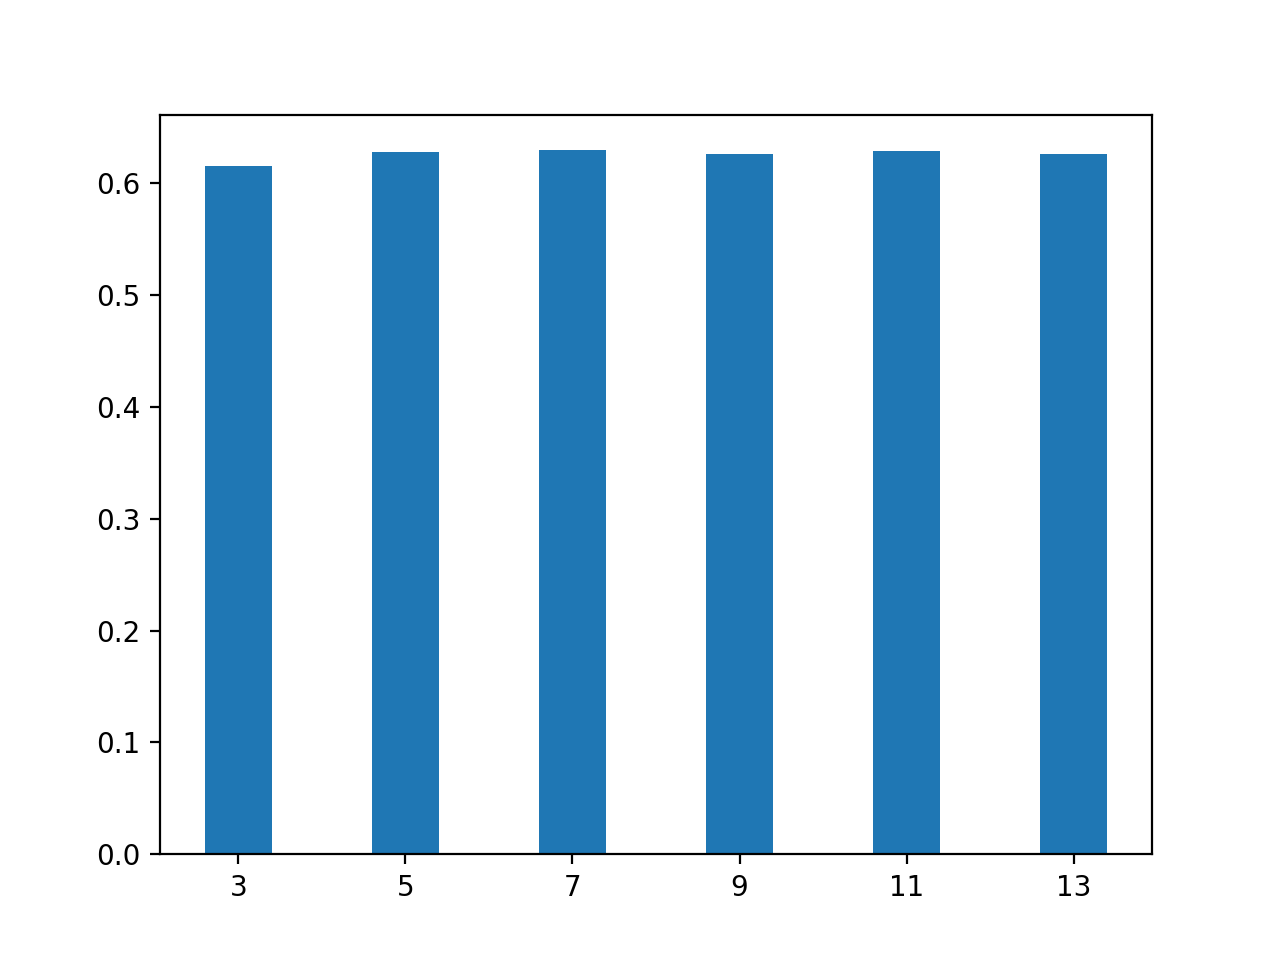
\includegraphics[width=\linewidth]{figures/knn_bar.png}
  \end{subfigure}
  \caption{KNN Bar}
  \label{fig:knn_bar}
\end{figure}

\item
Linear Regression Model Fitting

2.2



\item
Sample Exam Questions

3.1

The mean squared training error is $0$

\medskip
3.2

(a)

$$ (1^2 + (\frac{2}{3})^2 + 2^2) / 3 = 1.81 $$

(b)

$$ (1^2 + 0.5^2 + 0.5^2) / 3 = 0.5 $$

(c)

Will choose (b)

\medskip
3.3

(e)

A, because with more training data it becomes harder to well fit all records, it is more likely to make errors.

(f)

B, because more training data can represent the real data distribution better, the left testing data is more likely have been covered in the training.


% ========== Continue adding items as needed

\end{enumerate}

\end{document}
\grid
\grid
